%!TEX root = ./thesis-main.tex
%-------------------------------------------------------------------------------
%                            BAB IV
%         		ANALISIS DAN RANCANGAN SISTEM
%-------------------------------------------------------------------------------

\chapter{ANALISIS DAN RANCANGAN SISTEM}
	\section{Gambaran Umum Sistem}
	Penelitian ini ditujukan untuk memberikan informasi tentang Kota Palembang berdasarkan input \emph{NLP} dari pengguna. Sistem menerima input berupa \emph{query} bahasa alami dalam bahasa Indonesia. Sistem memproses input untuk dipahami dan hasilnya digunakan untuk melakukan pencarian informasi. Hasil pencarian informasi kemudian disajikan kepada pengguna.

	Data informasi fasilitas publik kota Palembang didapatkan dari \emph{Foursquare API} serta \emph{Google API} dalam format \emph{JSON}. Data tersebut akan diubah kedalam format \emph{RDF} agar dapat di akses menggunakan \emph{SPARQL Query}.Setiap tahapan proses yang dikerjakan sistem menggunakan basis pengetahuan yang direpresentasikan ke dalam 2 ontologi, yaitu ontologi Bahasa untuk merepresentasikan pengetahuan dibidang linguistik dan ontologi Informasi Publik Kota Palembang. Ontologi bahasa yang akan digunakan menggunakan ontologi yang telah dibuat sebelumnya oleh Admojo (2015) dan kemudian di tambahkan kosakata baru berkaitan informasi publik kota Palembang dikarenakan kosakata pada ontologi tersebut ditujukan untuk domain pendakian.
	
	Beberapa input yang dapat diproses dalam penelitian ini:
	\begin{enumerate}[a.]
		\item Carikan Hotel dalam radius 2 km dari Bandara
		\item Lokasi GOR Jakabaring Palembang
		\item Tampilkan daftar Event pada tanggal 16 November 2017
	\end{enumerate}
	
	Setelah input diterima akan dilakukan proses \emph{tokenizing}. Kata-kata yang telah di-\emph{tokenize} akan diubah menjadi bentuk kata baku, serta diperiksa \emph{spelling} dari setiap kata tersebut dengan membandingkan dengan data yang ada pada ontologi bahasa. Pada tahapan berikutnya, kata-kata tersebut akan diklasifikasikan ke dalam kelas-kelas seperti \emph{Event}, \emph{StopPoint}, \emph{ReligiousPlaces}, \emph{Shops}, dsb. Berdasarkan hasil kategori yang didapat kemudian dibuat \emph{query SPARQL} ke ontologi Informasi Publik Kota Palembang sehingga dihasilkan informasi yang dibutuhkan.
	
	\section{Desain Sistem}
	Sistem yang dikembangkan pada penelitian ini merupakan sistem berbasis web. Pengguna dapat melakukan pencarian informasi fasilitas publik kota Palembang  menggunakan web browser dengan input berupa bahasa alami yaitu bahasa Indonesia. Untuk memproses input hingga menghasilkan informasi, sistem terbagi menjadi dua komponen yaitu: \emph{Query Preprocessing} dan \emph{Query Mapping}. 
	
	Secara umum tahapan kerja sistem yang diusulkan ditunjukkan pada Gambar \ref{fig:arsitektur}.
	
	\begin{figure}[H]
		\centering
		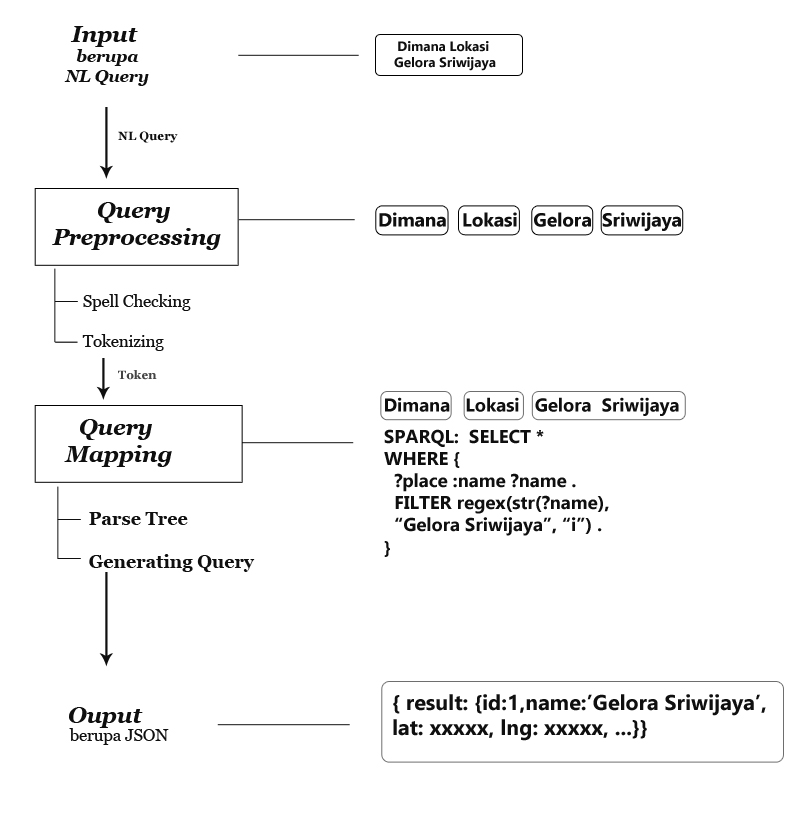
\includegraphics[scale=0.50]{gambar/arsitektur.png}
		\caption{Ilustrasi tahapan kerja sistem yang diusulkan}
		\label{fig:arsitektur}
	\end{figure}
	
	
	\subsection{\emph{Query Preprocessing}}
	Pada tahap \emph{Query Preprocessing} dilakukan validasi dan pengubahan input menjadi urutan kata (\emph{token}). Proses validasi dilakukan dengan memeriksa setiap kata input dengan kata yang terdapat dalam ontologi (ontologi Bahasa dan ontologi Informasi Publik Kota Palembang). Input dinyatakan valid apabila setiap token ada didalam ontologi. 
	
	Satuan kata pada urutan kata dapat mengandung satu kata atau lebih. Misalnya pada kata "Gelora" dan "Sriwijaya" seperti yang diilustrasikan pada Gambar \ref{fig:querypreprocessing}, berdasarkan pengetahuan pada ontologi Informasi Fasilitas Publik Kota Palembang, kata "Gelora Sriwijaya" merupakan nama untuk sebuah stadion yang berada di Kota Palembang. Oleh karena itu, sistem membakukan kata "Gelora" dan "Sriwijaya" menjadi "Gelora Sriwijaya".
	
	Proses pembentukan input menjadi urutan kata juga melibatkan pengambilan atribut tiap kata dari ontologi (ontologi Bahasa). Atribut tersebut yaitu Atribut Sintaksis yang digunakan untuk proses pengecekan sintaksis serta atribut semantik. 
	
	\begin{figure}[H]
		\centering
		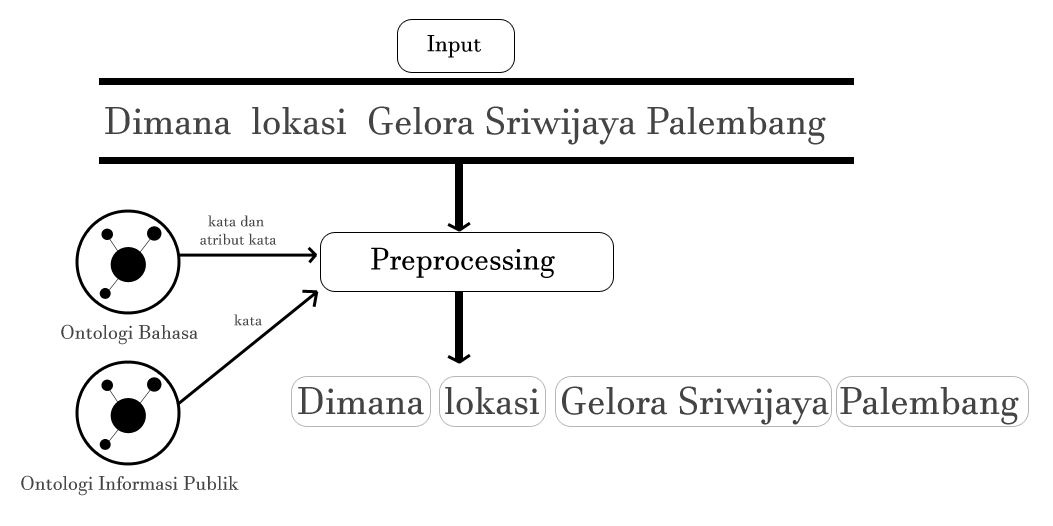
\includegraphics[scale=0.50]{gambar/querypreprocessing.png}
		\caption{Ilustrasi tahapan kerja sistem yang diusulkan}
		\label{fig:querypreprocessing}
	\end{figure}
	
	\subsection{\emph{Query Mapping}}
	Pada tahapan ini urutan \emph{token} yang didapatkan pada tahapan \emph{query preprocessing} di bentuk menjadi sebuah \emph{parse tree} dengan mencocokkan atribut sintaksis serta atribut semantik dari setiap \emph{token} menggunakan aturan-aturan tata bahasa Indonesia. Hasil dari \emph{parse tree} tersebut akan digunakan sebagai dasar pembentukan \emph{query SPARQL}. \emph{Query} dijalankan pada ontologi informasi publik kota Palembang sehingga menghasilkan jawaban dari \emph{query} yang diinput. Hasil jawaban dibentuk menggunakan format \emph{JSON} sehingga dapat di proses oleh \emph{client lintas platform}.
	
	Gambar \ref{fig:parsetree} menggambarkan pembentukan \emph{parse tree}.
	
	\begin{figure}[H]
		\centering
		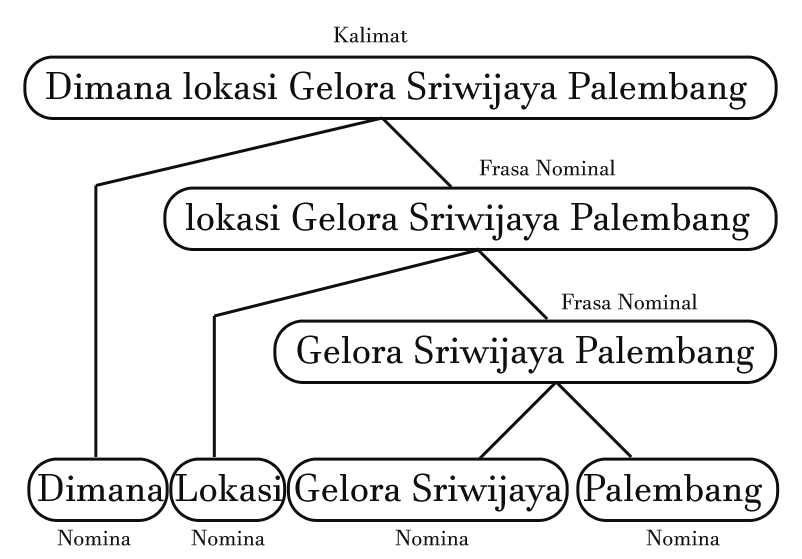
\includegraphics[scale=0.45]{gambar/parsetree.png}
		\caption{Ilustrasi pembentukan Parse Tree}
		\label{fig:parsetree}
	\end{figure}
	
	\section{Perancangan Ontologi}
	
	\subsection{Ontologi Bahasa}
	Pengetahuan bahasa yang digunakan dalam penelitian ini berkaitan dengan pengetahuan bidang linguistik yakni meliputi pengetahuan tentang kata, hubungan kata, kategori kata, fungsi sintaksis, dan perilaku semantik dari satuan bahasa. Pengetahuan sintaksis dan pengetahuan semantik digunakan pada proses pemahaman input menggunakan tata bahasa Indonesia baku yang dikemukakan oleh Alwi dkk., (2003).
	
	Pengetahuan sintaksis dan pengetahuan semantik dinyatakan dalam aturan-aturan gramatikal yang direpresentasikan menggunakan \emph{Unification Based Grammar} berdasarkan formalisme penulisan gramatikal yang telah dikemukakan oleh (Suryawan, 2013; Gazdar dan Mellish, 1989). 
	
	Pengetahuan pada ontologi Bahasa dideskripsikan ke dalam konsep konsep yang disusun berdasarkan suatu klasifikasi dan dikelompokkan ke dalam \emph{class-class} yang sama. Konsep yang digunakan pada ontologi Bahasa didasarkan pada konsep bahasa yang telah dideskripsikan oleh Suryawan (2013), yang dikembangkan sesuai dengan kebutuhan sistem pada penelitian ini.
	
	Pada penelitian ini digunakan ontologi bahasa yang telah dibuat sebelumnya pada penelitian Admojo (2013). Ontologi tersebut dikembangkan dengan menambahkan kata-kata baru yang berkaitan dengan informasi publik kota Palembang. Ontologi sebelumnya difokuskan pada kata-kata yang berkaitan dengan istilah-istilah \emph{mountaineering} sehingga perlu ditambahkan kosa kata baru yang dibutuhkan pada penelitian ini.
	
	Class yang dibentuk dalam ontologi Bahasa yaitu \emph{Lexicon}, \emph{WordCategory}, \emph{Semantic}, \emph{SemanticType}, \emph{QueryLogic}. Setiap class berada dalam domain yang sama, namun menyimpan konsep pengetahuan yang berbeda-beda. Hirarki antar class dideskripsikan pada Gambar \ref{fig:classontologibahasa}.
	
	\begin{figure}[H]
		\centering
		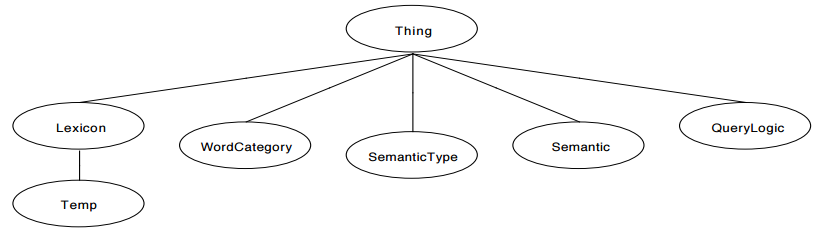
\includegraphics[scale=0.45]{gambar/classontologibahasa.png}
		\caption{\emph{Class-class} pada ontologi bahasa}
		\label{fig:classontologibahasa}
	\end{figure}
	
	Class Lexicon adalah representasi dari konsep kata yang merupakan satuan bahasa terkecil. Setiap individual yang terdapat di dalam class \emph{Lexicon} memiliki kategori, peran dan fungsi di dalam kalimat yang dideskripsikan menggunakan property, yaitu: \emph{word, category, semanticValue, type, argCat0, argCat1, argCat2, stripCat, argType0, argType1, argType2, stripType}. \emph{Property} yang digunakan untuk mendeskripsikan kata dijabarkan pada tabel 3.
	
	// tabel lagi disini
	
	Properti yang dijabarkan pada Tabel 3 memiliki fungsi, yaitu: Properti \emph{word} digunakan untuk mendeskripsikan struktur lahir suatu kata. Properti \emph{category} digunakan untuk mendeskripsikan kategori sintaksis yang dimiliki kata. Properti \emph{type} digunakan untuk mendeskripsikan tipe semantik yang dimiliki kata. Properti \emph{semanticValue} digunakan untuk mendeskripsikan nilai semantik kata Properti \emph{argCat0, argCat1, argCat2} dan \emph{stripCat} digunakan untuk mendeskripsikan hubungan perilaku sintaksis suatu kata, frasa, klausa, kalimat. Properti \emph{argType0, argType1, argType2} dan \emph{stripType} digunakan untuk mendeskripsikan hubungan perilaku semantik suatu kata, frasa, klausa, kalimat.
	
	\emph{Class SemanticType} merupakan realisasi dari konsep tentang perilaku semantik yang dimiliki oleh suatu kata. Konsep tentang perilaku semantik tidak dideskripsikan dengan menggunakan properti apapun.
	
	\emph{Class Semantic} merupakan realisasi dari konsep tentang nilai semantik dari suatu kata atau suatu satuan bahasa. Konsep tentang nilai semantik dari suatu kata atau suatu satuan bahasa tidak dideskripsikan dengan menggunakan properti apapun.
	
	\emph{Class WordCategory} merupakan realisasi dari konsep tentang kategori sintaksis. Konsep tentang kategori sintaksis tidak dideskripsikan dengan menggunakan properti apapun.
	
	\emph{Class QueryLogic} merupakan realisasi dari konsep informasi semantik dari suatu satuan bahasa. Konsep tentang makna dari suatu satuan bahasa dideskripsikan dengan menggunakan dua buah properti, yaitu: \emph{parA} dan \emph{qpart}. 
	
	\subsection{Ontologi Informasi Publik Kota Palembang}
	Ontologi informasi publik kota Palembang merupakan representasi dari pengetahuan tentang hal-hal yang dapat dicari oleh pengguna melalui sistem ini. Pengetahuan tersebut meliputi \emph{event-event} baik nasional maupun internasional yang diadakan di Palembang serta beberapa \emph{Point of Interest} yang meliputi tempat makan, tempat-tempat keagamaan, penginapan, toko, serta \emph{stop point} seperti halte \emph{busway}, halte \emph{LRT}, dsb. Gambar \ref{fig:classhierarchy} merupakan \emph{Class Hierarchy} yang akan digunakan pada sistem yang diusulkan.
	
	\begin{figure}[H]
		\centering
		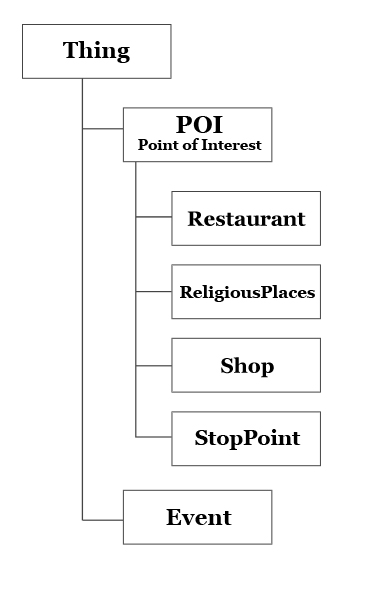
\includegraphics[scale=0.45]{gambar/classhierarchy.png}
		\caption{Struktur \emph{class hierarchy} sistem yang diusulkan}
		\label{fig:classhierarchy}
	\end{figure}
	
	Tabel menggambarkan properti minimum untuk mendeskripsikan konsep \emph{Point of Interest}
	
	

	\section{Perancangan Antarmuka}
		Habeo perfecto in sea. Ea deleniti gloriatur pri, paulo mediocrem incorrupte sea ei. Ad mollis scripta per. Incorrupte sadipscing ne mel. Mel ex nonumy malorum epicurei.

		Ne per tota mollis suscipit. Ullum labitur vim ut, ea dicit eleifend dissentias sit. Duis praesent expetenda ne sed. Sit et labitur albucius elaboraret. Ceteros efficiantur mei ad. Hendrerit vulputate democritum est at, quem veniam ne has, mea te malis ignota volumus.

		Eros reprimique vim no. Alii legendos volutpat in sed, sit enim nemore labores no. No odio decore causae has. Vim te falli libris neglegentur, eam in tempor delectus dignissim, nam hinc dictas an.
	
	\section{Subbab 2}		
		Habeo perfecto in sea. Ea deleniti gloriatur pri, paulo mediocrem incorrupte sea ei. Ad mollis scripta per. Incorrupte sadipscing ne mel. Mel ex nonumy malorum epicurei.

		\subsection{Subsubbab 2 1}
			Ne per tota mollis suscipit. Ullum labitur vim ut, ea dicit eleifend dissentias sit. Duis praesent expetenda ne sed. Sit et labitur albucius elaboraret. Ceteros efficiantur mei ad. Hendrerit vulputate democritum est at, quem veniam ne has, mea te malis ignota volumus.
			
			\begingroup
			    \fontsize{10pt}{12pt}\selectfont
			    \begin{verbatim}
					config mount
				        option target        /mnt
				        option device        /dev/sda1
				        option fstype        ext3
				        option options       rw,sync
				        option enabled       1
				        option enabled_fsck  0
				        option is_rootfs     1
			    \end{verbatim}  
			\endgroup

			\begingroup
			    \fontsize{10pt}{12pt}\selectfont
			    \begin{verbatim}
					# opkg update
					# opkg install python pyserial
			    \end{verbatim}  
			\endgroup			

		\subsection{Subsubbab 2 2}
			Consul graeco signiferumque qui id, usu eu summo dicunt voluptatum, nec ne simul perpetua posidonium. Eos ea saepe prodesset signiferumque. No dolore possit est. Mei no justo intellegebat definitiones, vis ferri lorem eripuit ad. Solum tritani scribentur duo ei, his an adipisci intellegat.

	\section{Subab 3}
		Consul graeco signiferumque qui id, usu eu summo dicunt voluptatum, nec ne simul perpetua posidonium. Eos ea saepe prodesset signiferumque. No dolore possit est. Mei no justo intellegebat definitiones, vis ferri lorem eripuit ad. Solum tritani scribentur duo ei, his an adipisci intellegat.
			
			
% Baris ini digunakan untuk membantu dalam melakukan sitasi.
% Karena diapit dengan comment, maka baris ini akan diabaikan
% oleh compiler LaTeX.
\begin{comment}
\bibliography{daftar-pustaka}
\end{comment}